% Tides above the Earth: a ring of freely falling particles, and each
% particle's acceleration relative to the ring's centre. In the Newtonian
% limit the relative acceleration of a particle displaced by (x, y) from the
% centre (y pointing away from the Earth) is (GM/r^3)(-x, 2y). The dashed
% ellipse is the ring a little later: stretched along y, squeezed along x.
\documentclass[tikz,border=1pt]{standalone}
% Shared preamble for the standalone figures: the book's fonts, palette and
% drawing styles. Figures are drawn at their final printed size. A column is
% 3.35in (241pt) wide; a figure across both columns is 7in (505pt) wide.

\usepackage[T1]{fontenc}
\usepackage{newpxtext}
\usepackage[varbb]{newpxmath}
\usepackage[semibold,scale=0.95,lining]{sourcesanspro}
\usepackage{xcolor}
% Palette shared by the book and by the standalone figures in figures/src.
% One main hue (blue), one accent (orange), and a few roles used sparingly.

\definecolor{seblue}{HTML}{1D5B8F}    % headings, worked examples, main curves
\definecolor{seblueDark}{HTML}{123E63}
\definecolor{seorange}{HTML}{DC7A26}  % thought experiments, light and light cones
\definecolor{seteal}{HTML}{1F8577}    % checks, travellers and ships
\definecolor{sered}{HTML}{C0392B}     % negative energy, tension, violations
\definecolor{seviolet}{HTML}{5E548E}  % going deeper
\definecolor{sesand}{HTML}{8C6A3F}    % history
\definecolor{segray}{HTML}{6B7480}    % axes, guides, secondary labels
\definecolor{selight}{HTML}{D5DAE1}   % grids and faint rules

\usepackage{siunitx}
\usepackage{fontawesome5}
\usepackage{tikz}
\usetikzlibrary{arrows.meta,calc,positioning,decorations.pathreplacing,
  decorations.markings,shapes.geometric,fadings,shadings,patterns,3d,
  intersections,backgrounds}
\usepackage{pgfplots}
\pgfplotsset{compat=1.18}
\usepgfplotslibrary{fillbetween,groupplots,colormaps}

\tikzset{
  >={Latex[length=2.1mm,width=1.4mm]},
  every picture/.style={line cap=round, line join=round},
  lbl/.style={font=\sffamily\footnotesize, text=black!85},
  smalllbl/.style={font=\sffamily\scriptsize, text=black!75},
  guide/.style={segray, line width=0.4pt},
  axisline/.style={segray, line width=0.5pt, -{Latex[length=1.7mm,width=1.1mm]}},
  light/.style={seorange, line width=0.9pt},
  lightdash/.style={seorange, line width=0.9pt, dash pattern=on 3pt off 2pt},
  ship/.style={seteal, line width=1.4pt},
  cone/.style={fill=seorange!22, draw=seorange!85!black, line width=0.35pt},
}

\pgfplotsset{
  se axis/.style={
    axis lines=left,
    axis line style={segray, line width=0.5pt, -{Latex[length=1.6mm,width=1.1mm]}},
    tick style={segray, line width=0.4pt},
    major tick length=2.5pt,
    tick label style={font=\sffamily\scriptsize, text=black!75},
    label style={font=\sffamily\footnotesize, text=black!85},
    every axis plot/.append style={line width=1.1pt},
    legend style={font=\sffamily\scriptsize, draw=none, fill=none},
    scaled ticks=false,
    xticklabel={\sansnum{\tick}}, yticklabel={\sansnum{\tick}},
  },
}

% Numbers in figures are set in the sans-serif text font, with a true minus.
\sisetup{mode=text, reset-text-family=false, reset-text-series=false,
  reset-text-shape=false, drop-zero-decimal, group-minimum-digits=5}
% Tick values arrive as long decimals (1.5000000000); parse them first.
\newcommand{\sansnum}[1]{\begingroup\pgfkeys{/pgf/fpu=false}%
  \pgfmathparse{1*(#1)}\num{\pgfmathresult}\endgroup}

\begin{document}
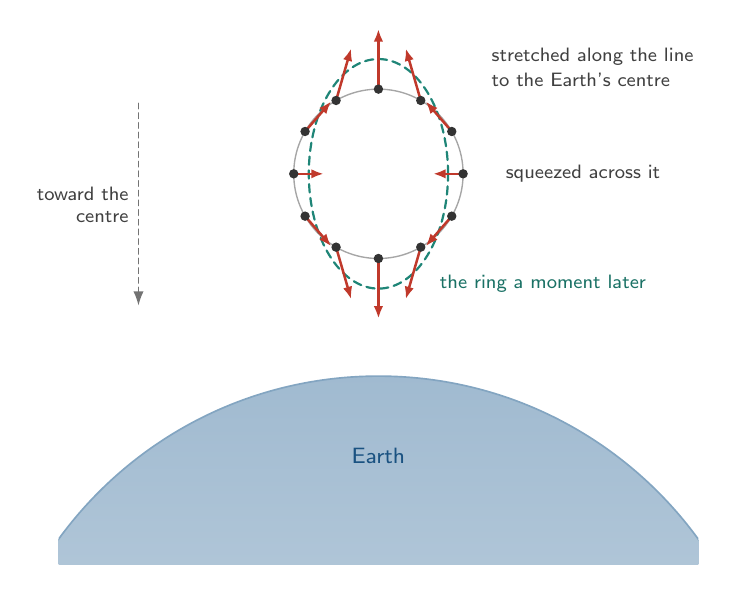
\begin{tikzpicture}[x=34pt, y=34pt]
% the Earth
\begin{scope}
  \clip (-3.4,-2.2) rectangle (3.4,0.2);
  \shade[top color=seblue!42, bottom color=seblue!14] (0,-4.4) circle (4.2);
  \draw[seblue!55, line width=0.6pt] (0,-4.4) circle (4.2);
\end{scope}
\node[lbl, text=seblue!90!black] at (0,-1.05) {Earth};
\draw[black!55, line width=0.5pt, -{Latex[length=1.8mm,width=1.3mm]}, dash pattern=on 2pt off 1.5pt]
  (-2.55,2.7) -- (-2.55,0.55) node[pos=0.5, anchor=east, smalllbl, align=right] {toward the\\centre};
% the ring and its later shape
\draw[black!35, line width=0.5pt] (0,1.95) circle (0.9);
\draw[seteal, line width=0.8pt, dash pattern=on 3pt off 2pt] (0,1.95) ellipse[x radius=0.74, y radius=1.22];
\foreach \a in {0,30,...,330} {
  \pgfmathsetmacro{\px}{0.9*sin(\a)}
  \pgfmathsetmacro{\py}{0.9*cos(\a)}
  \pgfmathsetmacro{\ax}{-0.32*sin(\a)}
  \pgfmathsetmacro{\ay}{0.64*cos(\a)}
  \draw[sered, line width=0.9pt, -{Latex[length=1.6mm,width=1.2mm]}]
    (\px,1.95+\py) -- ++(\ax,\ay);
  \fill[black!80] (\px,1.95+\py) circle (1.7pt);
}
\node[smalllbl, anchor=west] at (1.1,3.2) {stretched along the line};
\node[smalllbl, anchor=west] at (1.1,2.95) {to the Earth's centre};
\node[smalllbl, anchor=west] at (1.25,1.95) {squeezed across it};
\node[smalllbl, text=seteal!85!black, anchor=west] at (0.55,0.78) {the ring a moment later};
\end{tikzpicture}
\end{document}
